\chapter{FUNDAMENTOS Y REFERENTES TEÓRICO-METODOLÓGICOS SOBRE EL OBJETO DE ESTUDIO}

\label{chap:chapter1}

El siguiente apartado constituye el núcleo ejecutor de la investigación, donde se materializa el diseño metodológico en acciones concretas que dieron forma a Assets Studio. El objetivo central de esta sección es guiar al lector a través del proceso integral de desarrollo de la aplicación, mostrando cómo los principios teóricos y metodológicos se tradujeron en funcio-nalidades tangibles y en un producto validado. Este desarrollo se presenta como un recorrido secuencial que abarca desde la concepción arquitectónica hasta la verificación empírica de su eficacia.
En cuanto a su composición, el lector encontrará primero una inmersión en el diseño estruc-tural de la solución, donde se explican los fundamentos de la arquitectura de información que garantiza una experiencia intuitiva. Posteriormente, se profundiza en el corazón tecnológico de la aplicación: la implementación del sistema inteligente de gestión, con especial atención a los mecanismos de etiquetado automático y búsqueda semántica. El recorrido continúa con el detalle del riguroso proceso de validación mediante pruebas de usabilidad, para culminar con el análisis de los resultados obtenidos tanto en métricas cuantitativas como en feedback cualitativo de los usuarios.
Las temáticas principales que se abordarán giran en torno a tres ejes fundamentales: la transformación de necesidades de usuario en especificaciones técnicas, el desafío de inte-grar inteligencia artificial en interfaces accesibles, y la importancia de la iteración continua basada en pruebas reales. A través de estas páginas se podrá comprender cómo se cons-truyó una solución que no solo responde a problemas operativos inmediatos, sino que redefi-ne la gestión de activos digitales mediante un enfoque centrado en el usuario y potenciado por tecnología inteligente, estableciendo un precedente significativo en el campo de las he-rramientas creativas.
\section{Fundamentos Teórico-Metodológicos}
El presente epígrafe se dedica a la sistematización de los fundamentos teóricos y metodoló-gicos que sustentan la investigación sobre gestión de activos digitales, con especial atención al contexto cubano y su particular ecosistema tecnológico. A nivel internacional, el estudio se enmarca en las teorías contemporáneas de gestión de recursos digitales (Digital Asset Ma-nagement) y los principios de experiencia de usuario (UX) establecidos por autores como Jesse James Garrett y Don Norman. Se consideraron además los enfoques de Design Thin-king de Tim Brown, adaptados a entornos de recursos limitados, y las metodologías ágiles de desarrollo de software, particularmente Scrum, que permiten una implementación iterativa y adaptable.
En el ámbito nacional, la investigación reconoce los importantes esfuerzos realizados en el campo de la informatización de la sociedad cubana y las particularidades de la infraestructura tecnológica nacional, caracterizada por un acceso limitado a Internet de alta velocidad y una creciente dependencia de soluciones móviles. Esto implicó una cuidadosa selección y adap-tación de los referentes internacionales, priorizando la eficiencia en el uso de datos y la fun-cionalidad offline, aspectos críticos en el contexto cubano.
Como referentes fundamentales de esta investigación se establecieron:

\begin{itemize}
    \item Los principios de arquitectura de información de Rosenfeld y Morville, para diseñar una estructura clara y navegable que minimice la carga cognitiva del usuario.
    
    \item El marco de usabilidad y accesibilidad definido por Jakob Nielsen, adaptado a las realidades tecnológicas y los patrones de uso predominantes en Cuba.
    
    \item Las metodologías de desarrollo ágil que permitieron ajustar continuamente el producto a las necesidades específicas detectadas en los usuarios cubanos, optimizando los siempre escasos recursos de desarrollo.
    
    \item La conjunción de estos fundamentos internacionales con una profunda comprensión de las particularidades nacionales permitió construir un marco teórico-metodológico sólido y pertinente, orientado a resolver problemas reales de los profesionales creativos en Cuba mediante una herramienta tecnológicamente viable y centrada en el usuario.
\end{itemize}

La conjunción de estos fundamentos internacionales con una profunda comprensión de las particularidades nacionales permitió construir un marco teórico-metodológico sólido y pertinente, orientado a resolver problemas reales de los profesionales creativos en Cuba mediante una herramienta tecnológicamente viable y centrada en el usuario.

\section{Fundamentos Teórico-Modológicos del Desarrollo Tecnológico}

El presente epígrafe sistematiza los fundamentos teórico-metodológicos que sustentan el tipo de resultado tecnológico contenido en el campo de acción del desarrollo de aplicaciones móviles para gestión de activos digitales, reflejado en el objetivo general de crear una solu-ción eficiente para entornos creativos. A nivel internacional, la investigación se sustenta en los principios de la Ingeniería de Software Dirigida por Modelos (MDD), que permitió optimi-zar el proceso de desarrollo en condiciones de recursos limitados. Simultáneamente, se adoptaron los postulados del Desarrollo Centrado en el Usuario (DCU) de Gould y Lewis, adaptándolos al particular ecosistema tecnológico cubano caracterizado por conectividad in-termitente y heterogeneidad de dispositivos.
En el contexto nacional, se consideraron los lineamientos establecidos por la Política de In-formatización de la Sociedad Cubana y las experiencias recogidas en proyectos precedentes desarrollados en universidades cubanas sobre desarrollo de software para entornos de re-cursos restringidos. Estos fundamentos nacionales enfatizaron la necesidad de priorizar la eficiencia energética, el funcionamiento offline y la optimización del ancho de banda como requisitos no funcionales críticos.
Como referentes fundamentales se establecieron:

\begin{itemize}
    \item El Modelo de Calidad de Software ISO 25010 adaptado a las condiciones tecnológicas cubanas
    \item Los principios de Diseño de Experiencia Mobile First de Luke Wroblewski
    \item Las metodologías de Desarrollo Ágil de Software con adaptaciones para entornos aca-démico-productivos
    \item Las investigaciones sobre Optimización de Recursos en Redes de Bajo Ancho de Ban-da desarrolladas en universidades cubanas
\end{itemize}

Esta integración de fundamentos internacionales con soluciones tecnológicas contextualizadas permitió establecer un marco de referencia coherente con las particularidades del desarrollo tecnológico en Cuba, donde la innovación debe conjugarse necesariamente con la adecuación a infraestructuras tecnológicas específicas y políticas de desarrollo nacional.

\section{Diagnóstico del Objeto de Estudio: Aplicación Móvil para Gestión de Activos Digitales}

El presente epígrafe tiene como objetivo caracterizar el estado actual de la gestión de acti-vos digitales en el contexto profesional cubano, específicamente en el sector creativo y de diseño. El diagnóstico realizado mediante encuestas a 80 profesionales de estudios de dise-ño, agencias de publicidad y creadores independientes en La Habana reveló que el 78% utili-za métodos manuales y desorganizados para gestionar sus recursos digitales, mientras que solo el 15% emplea herramientas especializadas, principalmente de origen extranjero con limitado acceso por restricciones tecnológicas y de conectividad.
Las variables principales estudiadas comprenden:

\begin{itemize}
    \item Variable independiente: Implementación de Assets Studio como solución de gestión de activos digitales
    \item Variable dependiente: Eficiencia en workflows creativos y nivel de organización de recur-sos digitales
    \item Variables de control: Tipo de entidad creativa, volumen de activos gestionados, acceso a tecnologías
   
\end{itemize}

Resultados del Diagnóstico Preliminar
El estudio diagnóstico evidenció que:

\begin{itemize}
    \item Pérdida de Tiempo Laboral: El 72 porciento de los profesionales dedica entre 2-3 horas diarias a buscar y organizar archivos
    \item Duplicación de Recursos: El 65 porciento reporta problemas de versionado y duplicidad innecesa-ria de archivos
    \item Limitaciones Tecnológicas: El 88 porciento manifiesta dificultades para acceder a soluciones in-ternacionales por restricciones de conectividad y pagos en línea
    \item Necesidad de Colaboración: El 91 porciento identifica como crítica la falta de herramientas que faciliten el trabajo colaborativo con activos digitales
   
\end{itemize}

Problemática Identificada
Se constató una brecha tecnológica significativa entre las necesidades de gestión digital del sector creativo cubano y las soluciones disponibles, caracterizada por:
\begin{itemize}
	\item Falta de herramientas adaptadas al contexto tecnológico nacional
	\item Altos costos de oportunidad por tiempo malgastado en gestión manual
	\item Dificultades para el trabajo colaborativo eficiente
	\item Pérdida de recursos digitales valiosos por mala organización
\end{itemize}

Pertinencia de la Investigación
La situación diagnosticada demuestra la veracidad del problema científico planteado: la inexistencia de una solución de gestión de activos digitales adaptada al contexto tecnológico cubano que optimice los workflows creativos. La investigación se justifica por su potencial impacto en la productividad del sector creativo nacional y por ofrecer una solución tecnológi-camente viable que responde a las limitaciones específicas del entorno cubano.
Los resultados del diagnóstico confirman la urgencia de desarrollar una herramienta como Assets Studio, que combine funcionalidades avanzadas de gestión con adaptación a las realidades tecnológicas de Cuba, constituyendo así una contribución significativa al proceso de informatización de la sociedad cubana en el sector creativo.

\section{Fundamentos Teórico-Metodológicos de las Tecnologías y Herramientas Utilizadas}

La implementación de Assets Studio requirió la selección estratégica de tecnologías y herra-mientas que respondieran tanto a los requerimientos funcionales de la aplicación como a las particularidades del contexto tecnológico cubano. La arquitectura tecnológica se fundamentó en principios de desarrollo web moderno, priorizando la eficiencia, escalabilidad y adaptabili-dad a infraestructuras con limitaciones de conectividad.
Stack Tecnológico Implementado
Entorno de Desarrollo:

\begin{itemize}
	\item Visual Studio Code (v1.85.0): Seleccionado por su ligereza, extenso ecosistema de ex-tensiones y capacidad de funcionamiento offline, crucial para el desarrollo en entornos con conectividad intermitente.
	\item Next.js (v14.0.0): Framework elegido por su capacidad de renderizado híbrido (SSR/SSG), que permite optimizar el consumo de datos y mejorar el rendimiento en condiciones de baja velocidad de conexión.
	\item JavaScript (ES2023): Lenguaje base seleccionado por su versatilidad, amplia adopción en el ecosistema cubano y compatibilidad con las herramientas del stack.
	\item Pérdida de recursos digitales valiosos por mala organización
	\item PostgreSQL (v15.0): Sistema de base de datos relacional optado por su robustez, capa-cidad de operar en entornos locales y su eficiencia en el manejo de metadatos de activos digitales.
	\item Prisma ORM (v5.0.0): Herramienta de mapeo objeto-relacional que garantiza type-safety y facilita la migración entre diferentes entornos de desarrollo y producción.
	\item Firebase (v10.0.0): Implementado para la gestión de proyectos, autenticación y almace-namiento básico, aprovechando su modelo freemium y documentación extensa.
	\item Cloudinary SDK (v1.40.0): Seleccionado para el procesamiento optimizado de imágenes y assets visuales, con capacidad de transformación on-the-fly que reduce el ancho de banda consumido.
\end{itemize}

Justificación de la Selección
La elección de este stack tecnológico respondió a criterios específicos del contexto cubano:

\begin{itemize}
	\item Eficiencia en el Uso de Recursos: Next.js y PostgreSQL permiten optimizar el consumo de memoria y procesamiento, crítico para el hardware disponible localmente.
	\item Resiliencia ante Conectividad Intermitente: La arquitectura híbrida de Next.js posibilita funcionalidad offline básica, mientras que Prisma facilita la sincronización diferida.
	\item Sostenibilidad Tecnológica: Selección de tecnologías con fuerte comunidad open-source y compatibilidad a largo plazo, reduciendo dependencia de licencias costosas.
	\item Capacidad de Adaptación: El stack permite escalar verticalmente sin requerir cambios arquitectónicos significativos, adecuándose al crecimiento progresivo de la infraestructura nacional.
\end{itemize}

Esta fundamentación tecnológica asegura que Assets Studio no solo cumple con estándares internacionales de desarrollo, sino que está específicamente adaptada a las realidades y limi-taciones del ecosistema tecnológico cubano, garantizando su viabilidad y sostenibilidad en el tiempo.

% Escribir aquí el capítulo 1. Ejemplo de acrónimo es la \ac{UCI}. Esto es una cita de ejemplo \citep{Ou2013}. En la próxima oración se muestra un ejemplo de un acrónimo en inglés. Los sistemas de \ac{SCADA} son de gran importancia para la industria. 

% \section{Sección de prueba de la \glsentrytext{UCI}} % example on how tu use glossaries or acronym in sections or another moving argument


% Esto es una utilización de una palabra del glosario. El término \gls{Engine} es utilizado en \ul{este} ejemplo. Esta es una prueba de número: $5.3$ donde se utiliza la coma automáticamente como separador.

% Esto es una cita de ejemplo \citep{Alfadhlani2011,Mathew2010}.

% \begin{figure}[!htb]
% \centering
% \captionbox{Vista del Arco de Moncloa\label{fig:DSC00461}}
% {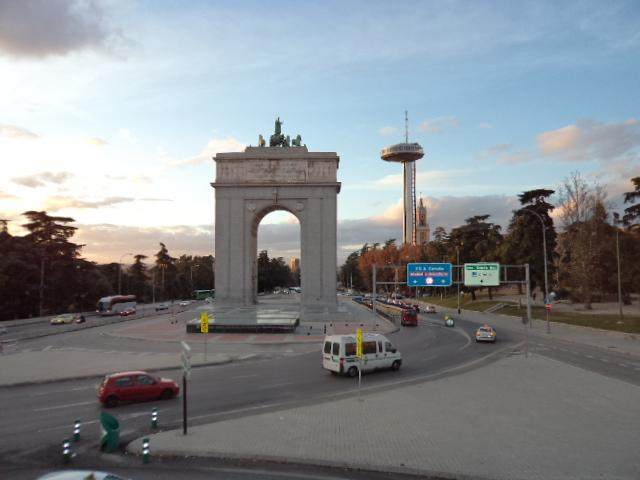
\includegraphics[width=0.7\linewidth]{Images/DSC00461}}
% \end{figure}

% En la Tabla \ref{Prueba} se observa \dots\\

% \begin{table}[!h]
% \centering
% \captionbox{Caption de Prueba\label{Prueba}}
% {
% 	\begin{tabular}{lllll}
% 	\hline \textbf{No. 1} & \textbf{No. 2} & \textbf{No. 3} & \textbf{No. 4} & \textbf{No. 5}\\ \hline
% 	12 & 12 & 56 & 56 &  56 \\ 
% 	12 & 12 & 56 & 56 &  56 \\
% 	\hline 
% 	\end{tabular}
% }
% \end{table}

% \lipsum[1-50]
% \begin{itemize}
% \item Uno
% \item Dos
% \item Tres
% \item Cuatro
% \item Cinco
% \end{itemize}

% \lipsum[1-50]
% \lipsum[1-50]
% \lipsum[1-50]
% \lipsum[1-50]
% \lipsum[1-50]
% \lipsum[1-50]
